\documentclass[dvipsnames,svgnames]{beamer}
\usetheme{Warsaw}
\usepackage[utf8]{inputenc}
\usepackage[english]{babel}
\usepackage{amsmath}
\usepackage{amsfonts}
\usepackage{amssymb}
\usepackage{graphicx}
\usepackage[linesnumbered,ruled]{algorithm2e}
\usepackage{tikz}
\usetikzlibrary{automata, positioning}
\usepackage{float}
\usepackage[normalem]{ulem}





\author{Charles Dufour}
\title{Reinforcement learning and robot navigation }
%\setbeamercovered{transparent} 
\setbeamertemplate{navigation symbols}{} 
%\logo{} 
%\institute{} 
%\date{} 
%\subject{} 

\newtheorem{madef}{Definition}

\begin{document}


\begin{frame}
\titlepage
\end{frame}

%\begin{frame}
%\tableofcontents
%\end{frame}



\begin{frame}
\frametitle{Introduction}
\begin{block}{The problem}

  \begin{itemize}
   \item Framework : the Disopt robot which can follow lines
   \item The problem : the robot should adapt its speed with           respect to traffic lights
   \item How : using Markov Decision Process (MDP) and Reinforcement Learning (RL)
  \end{itemize}
\end{block} 
\end{frame}


\begin{frame}
\frametitle{MDP Intuition}

\begin{figure}[ht]
\centering
    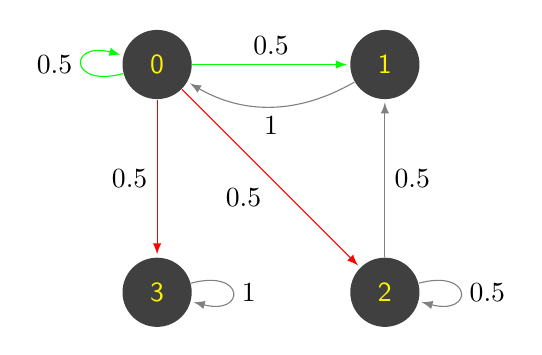
\begin{tikzpicture}[font=\sffamily]
    % Add the states
        \node[state,
              text=yellow,
              draw=none,
              fill=gray!50!black] (0) {0};
        \node[state,
              right=2cm of 0,
              text=yellow,
              draw=none, 
              fill=gray!50!black] (1) {1};
        \node[state,
              below=2cm of 1,
              text=yellow,
              draw=none, 
              fill=gray!50!black] (2) {2};
        \node[state,
        	  below = 2cm of 0,
        	  text=yellow,
        	  draw=none,
        	  fill=gray!50!black] (3) {3};
     

              
 \draw[every loop,
        auto=right,
        >=latex,
        draw=gray,
        fill=gray]
        
        	(0) edge[loop left, draw = green] node {$0.5$}(0)
        	(0) edge[ auto = right,draw = red]  node {$0.5$}(2)
        	(0) edge[auto = right,draw = red] node{$0.5$}  (3)
            (0) edge[auto = left,draw=green]  node {$0.5$} (1)
            (1) edge[bend left,auto =left]  node {$1$} (0)
            (2) edge[]  node {$0.5$}(1)
			(2) edge[loop right] node{$0.5$} (2)
			(3) edge[loop right] node{$1$} (3)	
			       
            ;       
      
    \end{tikzpicture}

\end{figure}
Sequence of events : $s_0,a_1,s_1,r_1,a_2,\ldots$

\end{frame}






\begin{frame}
\frametitle{MDPs}
\begin{block}{Definition }
\begin{itemize}
\item A set of states $\mathcal{S}=\{s_0,s_1,s_2,\ldots,s_{n}\}$
\item A set of actions $\mathcal{A}=\{a_1,a_2,a_3,\ldots,a_{k}\}$
\item A transition function $T(a,s,s') = \mathbb{P}[s'\mid a,s]$
\item A reward function $R: \mathcal{S}\mapsto \mathbb{R}$
\item A discount factor $0 \leq \gamma < 1$ 
\end{itemize}
\end{block}

\begin{block}{Markov Property}
The transitions only depends on the current state and the current action.
\end{block}
\end{frame}

%\begin{frame}
%\frametitle{to be told}
%Particularly, at each time step, our process is in some state $s$.\\Then our learning agent decides which action to execute from the set $\mathcal{A}$ which is doable from state $s$.\\Then the process moves randomly to a new state $s'$ following $T$ and gives the agent a reward $R(s')$.\\The purpose of our agent is to maximise the cumulative reward it gets in the long run.
%
%\end{frame}





\begin{frame}
\frametitle{how to pick actions}
\begin{madef}
A \emph{policy} $\pi$ is a probabilistic mapping from the set of states to the set of actions : 
$$ \pi : \mathcal{A} x \mathcal{S} \mapsto [0,1] $$
\\
s.t. $\underset{a}{\sum } \pi(a\mid s)=1 \quad \forall s \in \mathcal{S}$

\end{madef}
\end{frame}

\begin{frame}
\frametitle{Issue}
\begin{alertblock}{How to ?}
How to asses the goodness of policies so we can find the best one ? 

What is the best policy ?
\end{alertblock}
\end{frame}

\begin{frame}
\frametitle{how to asses the goodness of policies}
\begin{block}{We are interested in maximizing the discounted return}
$$ G_t= \sum_{k=0}^{\infty}\gamma^k R_{t+k+1} = R_{t+1} + \gamma G_{t+1}$$
\end{block}

\pause
\begin{block}{action value while in a state s under $\pi$}
\begin{equation}
q_{\pi}(s,a) = \mathbb{E}_{\pi}[G_t\mid S_t =s,A_t=a]
\end{equation}
\end{block}

\pause
\begin{block}{state value under policy $\pi$}
\begin{equation}
v_{\pi}(s)=\mathbb{E}_{\pi}[G_t \mid S_t=s]
\end{equation}
\end{block}



\end{frame}

\begin{frame}
\frametitle{Recursive definition of function values}
\begin{block}{action value}
\begin{equation}
\begin{split}
q_{\pi}(s,a) &= \mathbb{E}_{\pi}[G_t\mid S_t =s, A_t=a]
\\&=\mathbb{E}_{\pi}[R_{t+1}+\gamma G_{t+1}\mid S_t =s, A_t=a]
\\& =\sum_{s'}\mathbb{P}(s'\mid a,s)\left[r + \gamma \mathbb{E}_{\pi}\left[G_{t+1} \mid S_{t+1}=s' \right]\right]
\\& = \sum_{s'}\mathbb{P}(s'\mid a,s)\left[r + \gamma v_{\pi}(s') \right]
\end{split}
\end{equation}
\end{block}

with $r=R(s')$
\end{frame}


\begin{frame}
\frametitle{Recursive definition of function values}
\begin{block}{state value}
\begin{equation}
\begin{split}
v_{\pi}(s) &= \mathbb{E}_{\pi}[G_t\mid S_t =s]
\\&=\mathbb{E}_{\pi}[R_{t+1}+\gamma G_{t+1}\mid S_t =s]
\\& =\sum_{a }\pi(a \mid s) \sum_{s'}\mathbb{P}(s'\mid a,s)\left[r + \gamma \mathbb{E}_{\pi}\left[G_{t+1} \mid S_{t+1}=s' \right]\right]
\\& =\sum_{a }\pi(a \mid s) \sum_{s'}\mathbb{P}(s'\mid a,s)\left[r + \gamma v_{\pi}(s') \right]
\\&=\sum_{a }\pi(a \mid s)q_{\pi}(s,a)
\end{split}
\end{equation}
\end{block}

with $r=R(s')$
\end{frame}




\begin{frame}
\frametitle{how to asses the goodness of policies}
\begin{block}{how to compare two policies}
$$ \pi \leq \pi ' \iff  v_{\pi}(s) \leq v_{\pi'}(s) \quad \forall s \in \mathcal{S}
$$
\end{block}

\pause 

\begin{block}{Optimal policy}
$$ \pi_{*} \quad s.t. \quad \forall \pi : \pi_{*}\geq \pi $$
\end{block}
\end{frame}

%\begin{frame}
%\frametitle{Bellman optimality principle}
% An optimal policy has the property that whatever the initial state and initial decision are, the remaining decisions must constitute an optimal policy with regard to the state resulting from the first decision. (See Bellman, 1957, Chap. III.3.)
%\end{frame}

\begin{frame}
\frametitle{Bellman optimality equations}

The optimal policy $\pi_{*}$ has value functions  $v_*$ and $q_*$

\begin{block}{}

\begin{equation}
\begin{split}
v_{*}(s)&=\underset{a}{\text{max }} q_{\pi_{*}}(s,a)
\\&=\max_{a} \sum_{s'}\mathbb{P}(s'\mid s,a)[R(s')+\gamma v_{*}(s')]
\end{split}
\end{equation}
\end{block}

\begin{block}{}
\begin{equation}
\begin{split}
q_{*}(s,a)&=\mathbb{E}\left[ R_{t+1} + \gamma \max_{a'} q_{*}(S_{t+1},a') \mid S_t = s, A_t = a \right]
\\&= \sum_{s'}\mathbb{P}(s' \mid s,a)[R(s')+\gamma \max_{a'}q_{*}(s',a')]
\end{split}
\end{equation}
\end{block}

%Intuitively these equations say that the value of a state under the optimal policy must equal the expected return for the best action from that state. For finite MDPs these equations have a unique solution.
\end{frame}


\begin{frame}
\frametitle{finding optimal policy from value functions}
\begin{block}{}

$$\pi_{*}(s)= \underset{a}{\text{argmax }}q_*(s,a)$$
\end{block}
\end{frame}

\begin{frame}
\frametitle{Another issue}
\begin{alertblock}{computational issue}
If we wanted to solve these equations directly, it would cost a lot of computational power to know exactly the value functions first and then to solve since they are not linear. So how do we do it ? 
\end{alertblock}

\pause 
\vspace{1cm}
\centering
Approximation of value function

\end{frame}

\begin{frame}
\frametitle{solving MDPs using dynamic programming}
\begin{block}{iterative policy evaluation}
update rule : 
$$ v_{k+1}(s)=\sum_{a \in \mathcal{A}}\pi(a \mid s)\sum_{s',r}T(a,s,s')\left[r+\gamma v_k(s')\right] $$
\end{block}
\pause
\begin{block}{Policy Improvement}
$\pi/\pi'$ : old/new policy.
$$\pi'(s) = \underset{a \in \mathcal{A}}{\text{argmax } } q_{\pi}(s,a) $$
\end{block}

\end{frame}


\begin{frame}
\frametitle{Policy iteration algorithm}
%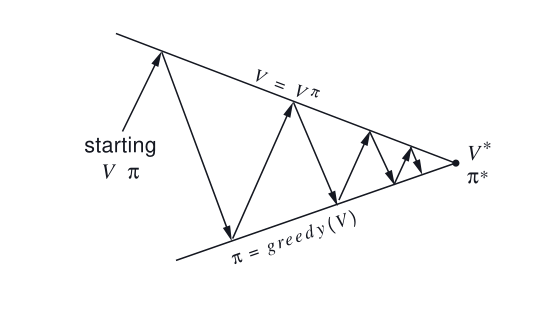
\includegraphics[scale=0.6]{img/generalized_policy_iter_sutton.png}
\centering
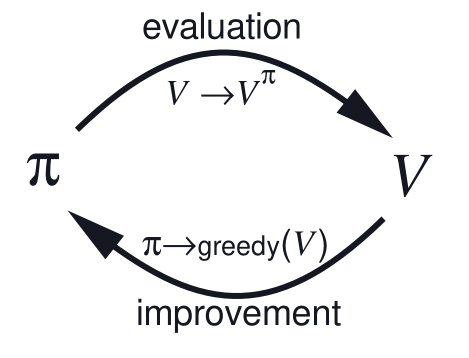
\includegraphics[scale=0.7]{img/policy_iter_sutton.png}
\footnote{From (Sutton \& Barto, 1998)}

\end{frame}


\begin{frame}
\frametitle{Our problem}
\begin{center}
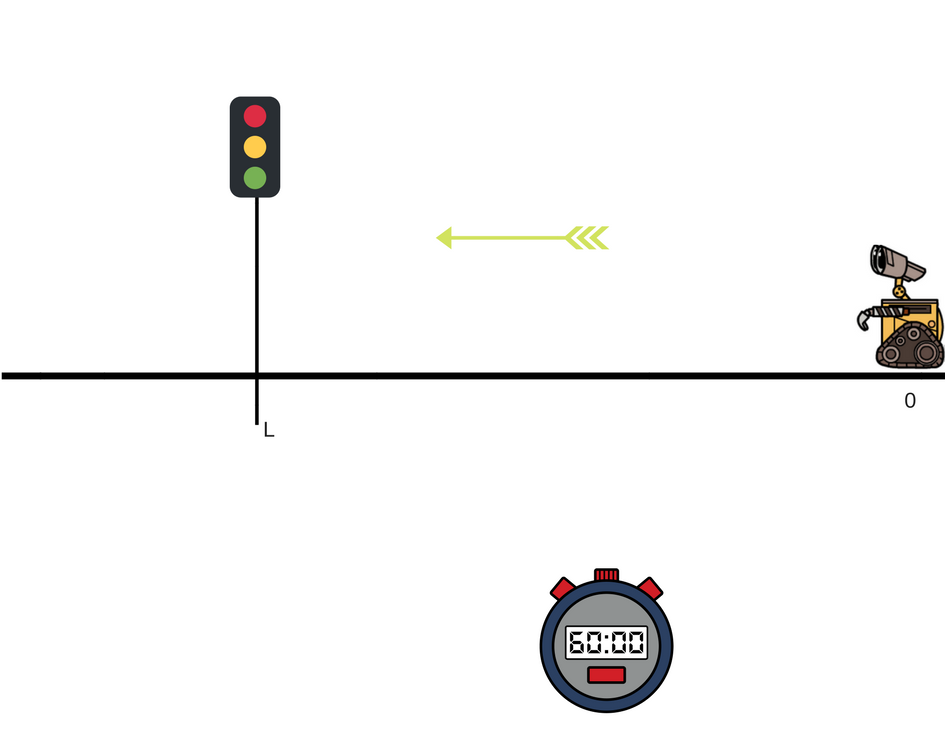
\includegraphics[scale=0.4]{img/illustration_traffic_light.png}
\end{center}
\end{frame}


\begin{frame}
\frametitle{First a simpler problem}
\begin{center}
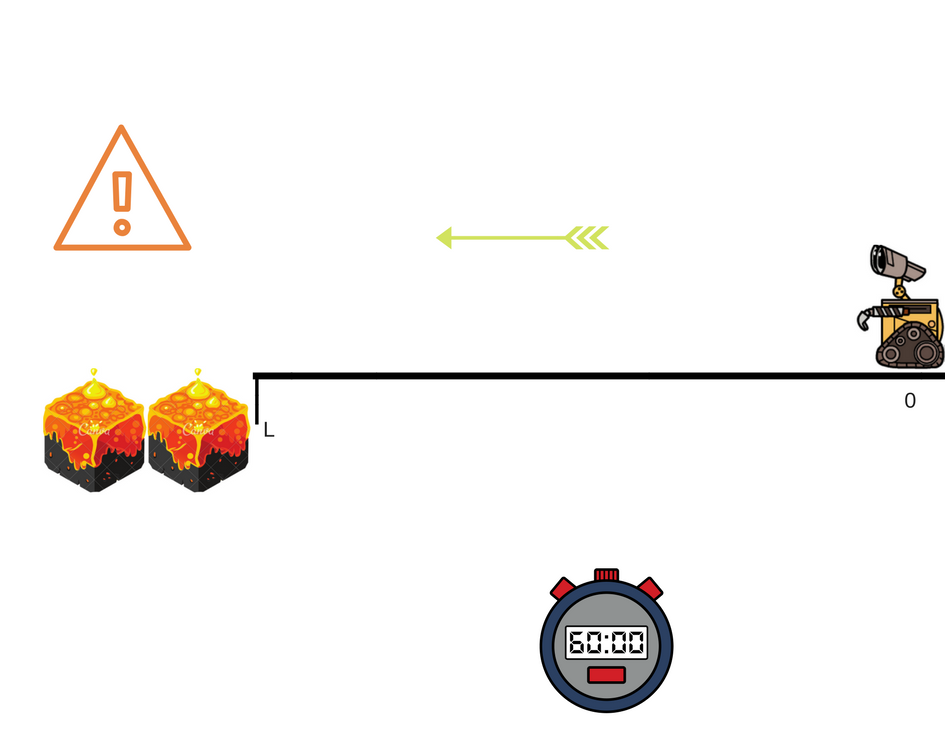
\includegraphics[scale=0.4]{img/illustration_lava.png}
\end{center}
\end{frame}

\begin{frame}
\frametitle{modelization}
\begin{block}{States}
\begin{itemize}
\item \pause position \{0,1,2,\ldots ,L, Lava  \}
\item \pause speed    \{low, medium, high   \}
\end{itemize}
\end{block}
\pause
\begin{block}{Actions}
\begin{itemize}
\item \pause decelerating 
\item \pause maintaining speed
\item \pause accelerating 
\end{itemize}
\end{block}
\end{frame}


\begin{frame}
\begin{center}
\frametitle{keeping the same speed graph}

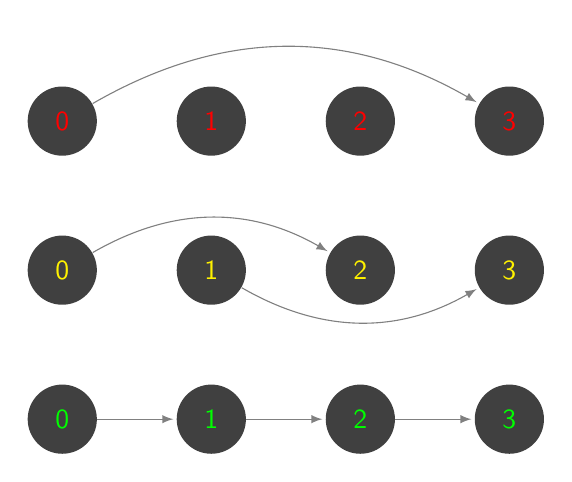
\begin{tikzpicture}[font=\sffamily]
    % Add the states
        \node[state,
              text=red,
              draw=none,
              fill=gray!50!black] (h0) {0};	
		\node[state,
			below=1 cm of h0,
        	text=yellow,
        	draw=none,
        	fill=gray!50!black] (m0) {0};
		\node[state,
			below= 1 cm of m0,
        	text=green,
        	draw=none,
        	fill=gray!50!black] (l0) {0};
         \node[state,
         	 right = 1 cm of h0,
              text=red,
              draw=none,
              fill=gray!50!black] (h1) {1};	
		\node[state,
			below=1 cm of h1,
        	text=yellow,
        	draw=none,
        	fill=gray!50!black] (m1) {1};
		\node[state,
			below= 1 cm of m1,
        	text=green,
        	draw=none,
        	fill=gray!50!black] (l1) {1};
         \node[state,
         	right = 1 cm of h1,
              text=red,
              draw=none,
              fill=gray!50!black] (h2) {2};	
		\node[state,
			below=1 cm of h2,
        	text=yellow,
        	draw=none,
        	fill=gray!50!black] (m2) {2};
		\node[state,
		below= 1 cm of m2,
        	text=green,
        	draw=none,
        	fill=gray!50!black] (l2) {2};
        \node[state,
        	right = 1 cm of h2,
              text=red,
              draw=none,
              fill=gray!50!black] (h3) {3};	
		\node[state,
			below=1 cm of h3,
        	text=yellow,
        	draw=none,
        	fill=gray!50!black] (m3) {3};
		\node[state,
			below= 1 cm of m3,
        	text=green,
        	draw=none,
        	fill=gray!50!black] (l3) {3};        	       	
			
		        
       \draw[every loop,
        auto=right,
        >=latex,
        draw=gray,
        fill=gray]
			(l0) edge[](l1)
			(l1) edge[] (l2)	
			(l2) edge[] (l3)
			(m0) edge[bend left] (m2)
			(m1) edge[bend right] (m3)
			(h0) edge[bend left] (h3)
	       
            ;
    \end{tikzpicture}
     \end{center}

 red : high speed \\ yellow : medium speed \\green : low speed

\end{frame}

\begin{frame}
\begin{center}
\frametitle{accelerating graph}
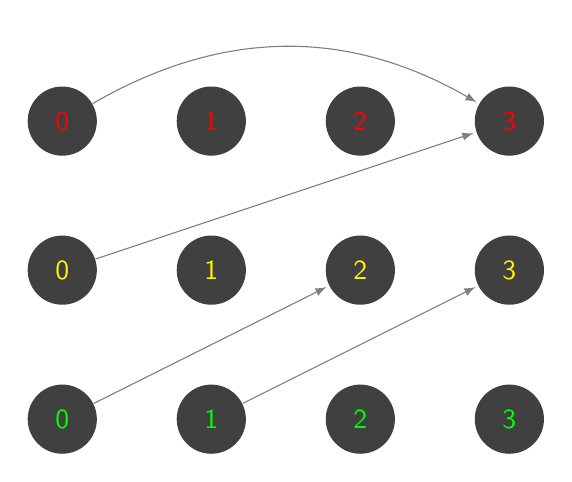
\begin{tikzpicture}[font=\sffamily]
    % Add the states
        \node[state,
              text=red,
              draw=none,
              fill=gray!50!black] (h0) {0};	
		\node[state,
			below=1 cm of h0,
        	text=yellow,
        	draw=none,
        	fill=gray!50!black] (m0) {0};
		\node[state,
			below= 1 cm of m0,
        	text=green,
        	draw=none,
        	fill=gray!50!black] (l0) {0};
         \node[state,
         	 right = 1 cm of h0,
              text=red,
              draw=none,
              fill=gray!50!black] (h1) {1};	
		\node[state,
			below=1 cm of h1,
        	text=yellow,
        	draw=none,
        	fill=gray!50!black] (m1) {1};
		\node[state,
			below= 1 cm of m1,
        	text=green,
        	draw=none,
        	fill=gray!50!black] (l1) {1};
         \node[state,
         	right = 1 cm of h1,
              text=red,
              draw=none,
              fill=gray!50!black] (h2) {2};	
		\node[state,
			below=1 cm of h2,
        	text=yellow,
        	draw=none,
        	fill=gray!50!black] (m2) {2};
		\node[state,
		below= 1 cm of m2,
        	text=green,
        	draw=none,
        	fill=gray!50!black] (l2) {2};
        \node[state,
        	right = 1 cm of h2,
              text=red,
              draw=none,
              fill=gray!50!black] (h3) {3};	
		\node[state,
			below=1 cm of h3,
        	text=yellow,
        	draw=none,
        	fill=gray!50!black] (m3) {3};
		\node[state,
			below= 1 cm of m3,
        	text=green,
        	draw=none,
        	fill=gray!50!black] (l3) {3};        	       	
			
		        
       \draw[every loop,
        auto=right,
        >=latex,
        draw=gray,
        fill=gray]
			(l0) edge[](m2)
			(l1) edge[] (m3)	
			(m0) edge[] (h3)
			(h0) edge[bend left] (h3)
	       
            ;
    \end{tikzpicture}
 \end{center}
\end{frame}


\begin{frame}
\begin{center}
\frametitle{decelerating}
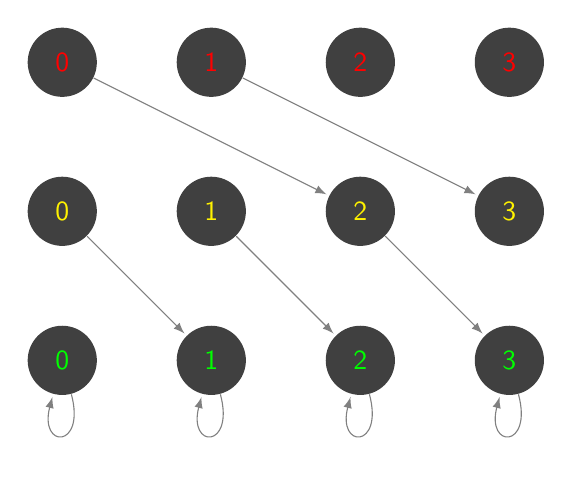
\begin{tikzpicture}[font=\sffamily]
    % Add the states
        \node[state,
              text=red,
              draw=none,
              fill=gray!50!black] (h0) {0};	
		\node[state,
			below=1 cm of h0,
        	text=yellow,
        	draw=none,
        	fill=gray!50!black] (m0) {0};
		\node[state,
			below= 1 cm of m0,
        	text=green,
        	draw=none,
        	fill=gray!50!black] (l0) {0};
         \node[state,
         	 right = 1 cm of h0,
              text=red,
              draw=none,
              fill=gray!50!black] (h1) {1};	
		\node[state,
			below=1 cm of h1,
        	text=yellow,
        	draw=none,
        	fill=gray!50!black] (m1) {1};
		\node[state,
			below= 1 cm of m1,
        	text=green,
        	draw=none,
        	fill=gray!50!black] (l1) {1};
         \node[state,
         	right = 1 cm of h1,
              text=red,
              draw=none,
              fill=gray!50!black] (h2) {2};	
		\node[state,
			below=1 cm of h2,
        	text=yellow,
        	draw=none,
        	fill=gray!50!black] (m2) {2};
		\node[state,
		below= 1 cm of m2,
        	text=green,
        	draw=none,
        	fill=gray!50!black] (l2) {2};
        \node[state,
        	right = 1 cm of h2,
              text=red,
              draw=none,
              fill=gray!50!black] (h3) {3};	
		\node[state,
			below=1 cm of h3,
        	text=yellow,
        	draw=none,
        	fill=gray!50!black] (m3) {3};
		\node[state,
			below= 1 cm of m3,
        	text=green,
        	draw=none,
        	fill=gray!50!black] (l3) {3};        	       	
			
		        
       \draw[every loop,
        auto=right,
        >=latex,
        draw=gray,
        fill=gray]
			(l0) edge[loop below](l0)
			(l1) edge[loop below] (l1)	
			(l2) edge[loop below] (l2)
			(l3) edge[loop below] (l3)
			(m0) edge[] (l1)
			(m1) edge[] (l2)
			(m2) edge[] (l3)
			(h0) edge[] (m2)
			(h1) edge[] (m3)
	       
            ;
    \end{tikzpicture}
 \end{center}
\end{frame}


\begin{frame}
\frametitle{Results}
\framesubtitle{States value evolution}
\begin{block}{}
\centering
States values at iterations $0,2,4$ and $6$ (where stable policy is attained)
\end{block}
\vspace{1cm}
\centering
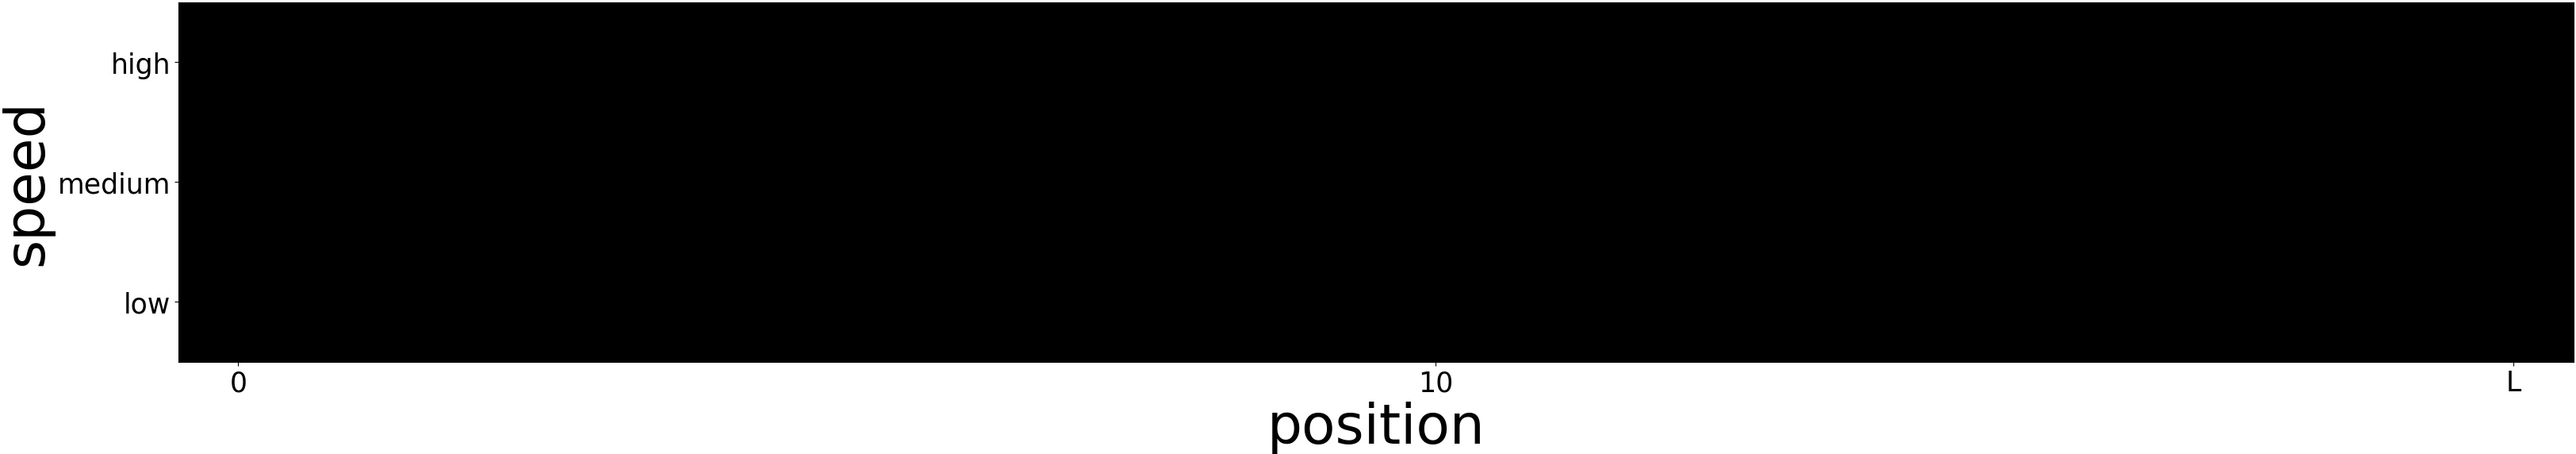
\includegraphics[scale=0.1]{img/value0.jpg}\\
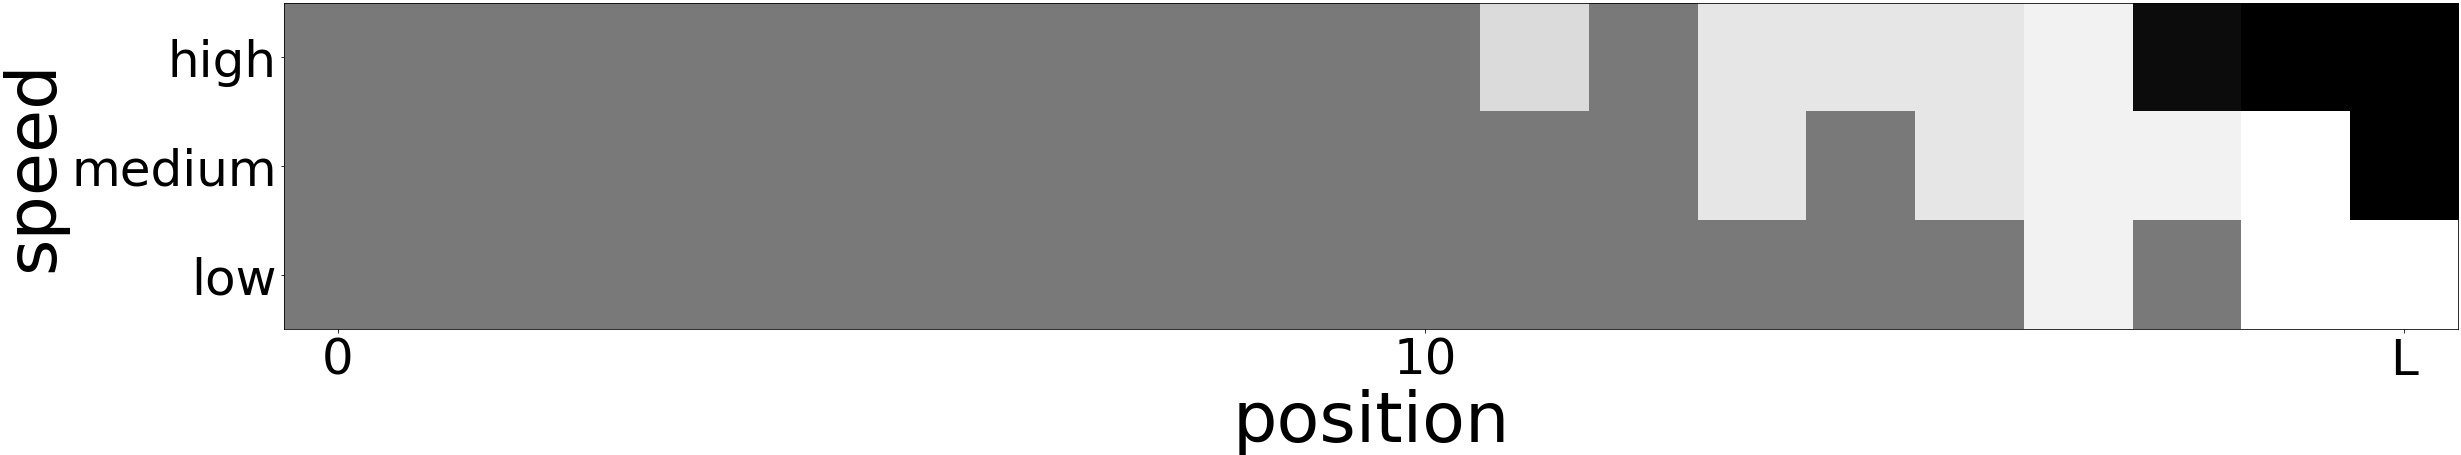
\includegraphics[scale=0.1]{img/value2.jpg}\\
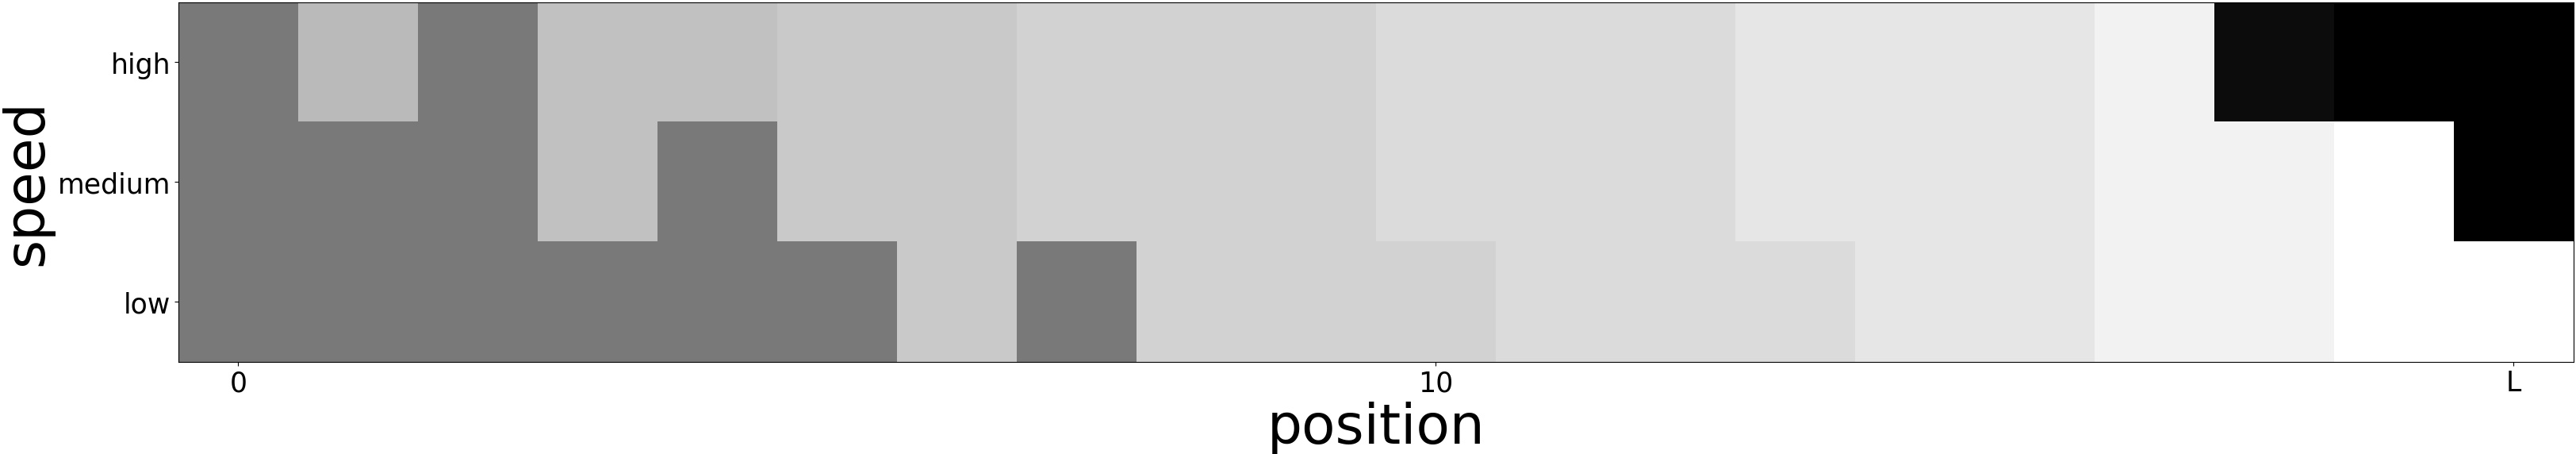
\includegraphics[scale=0.1]{img/value4.jpg}\\
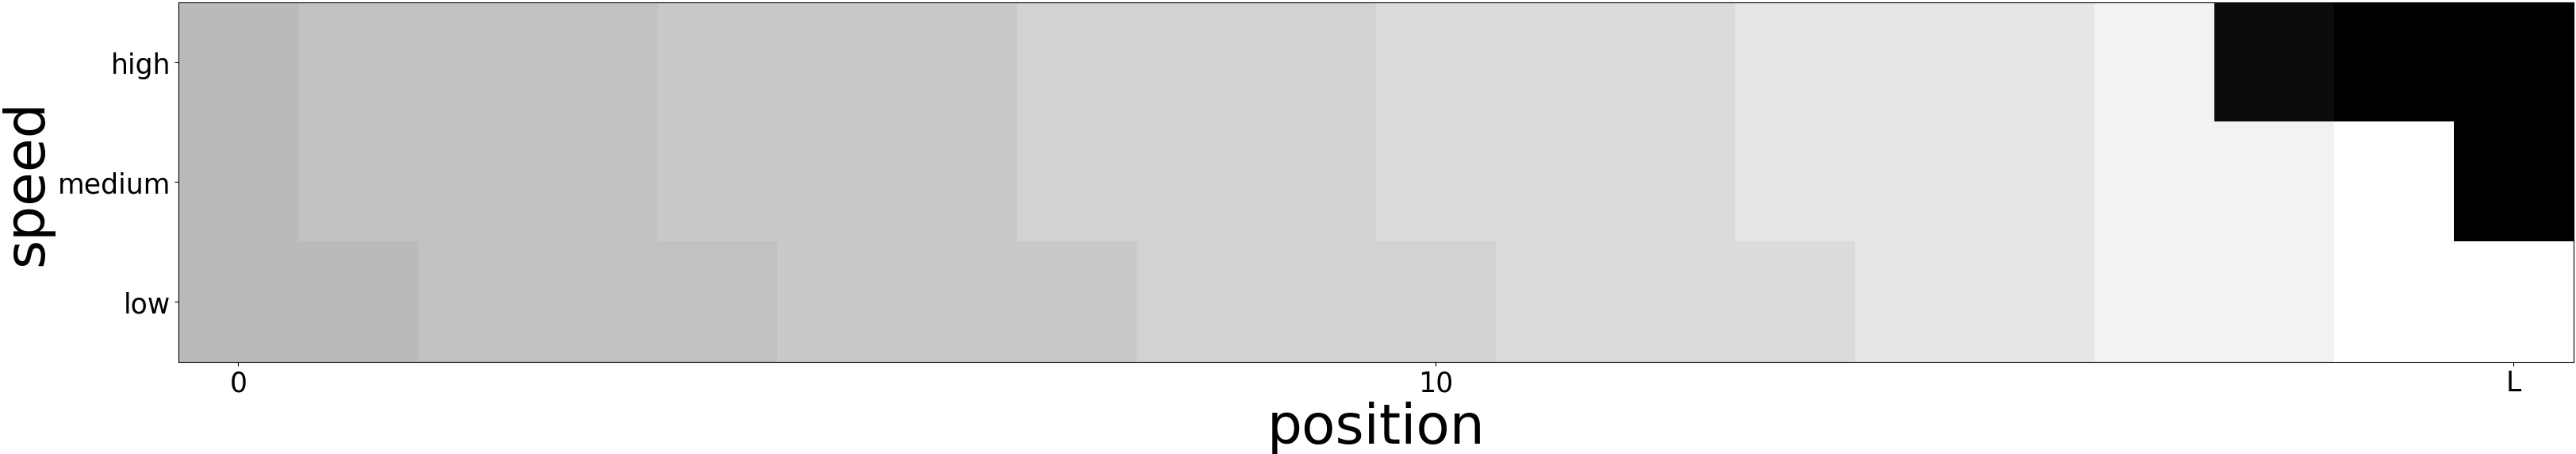
\includegraphics[scale=0.1]{img/value6.jpg}\\


\end{frame}


\begin{frame}
\frametitle{Results for deterministic actions}
\framesubtitle{One of the optimal trajectories}
\centering
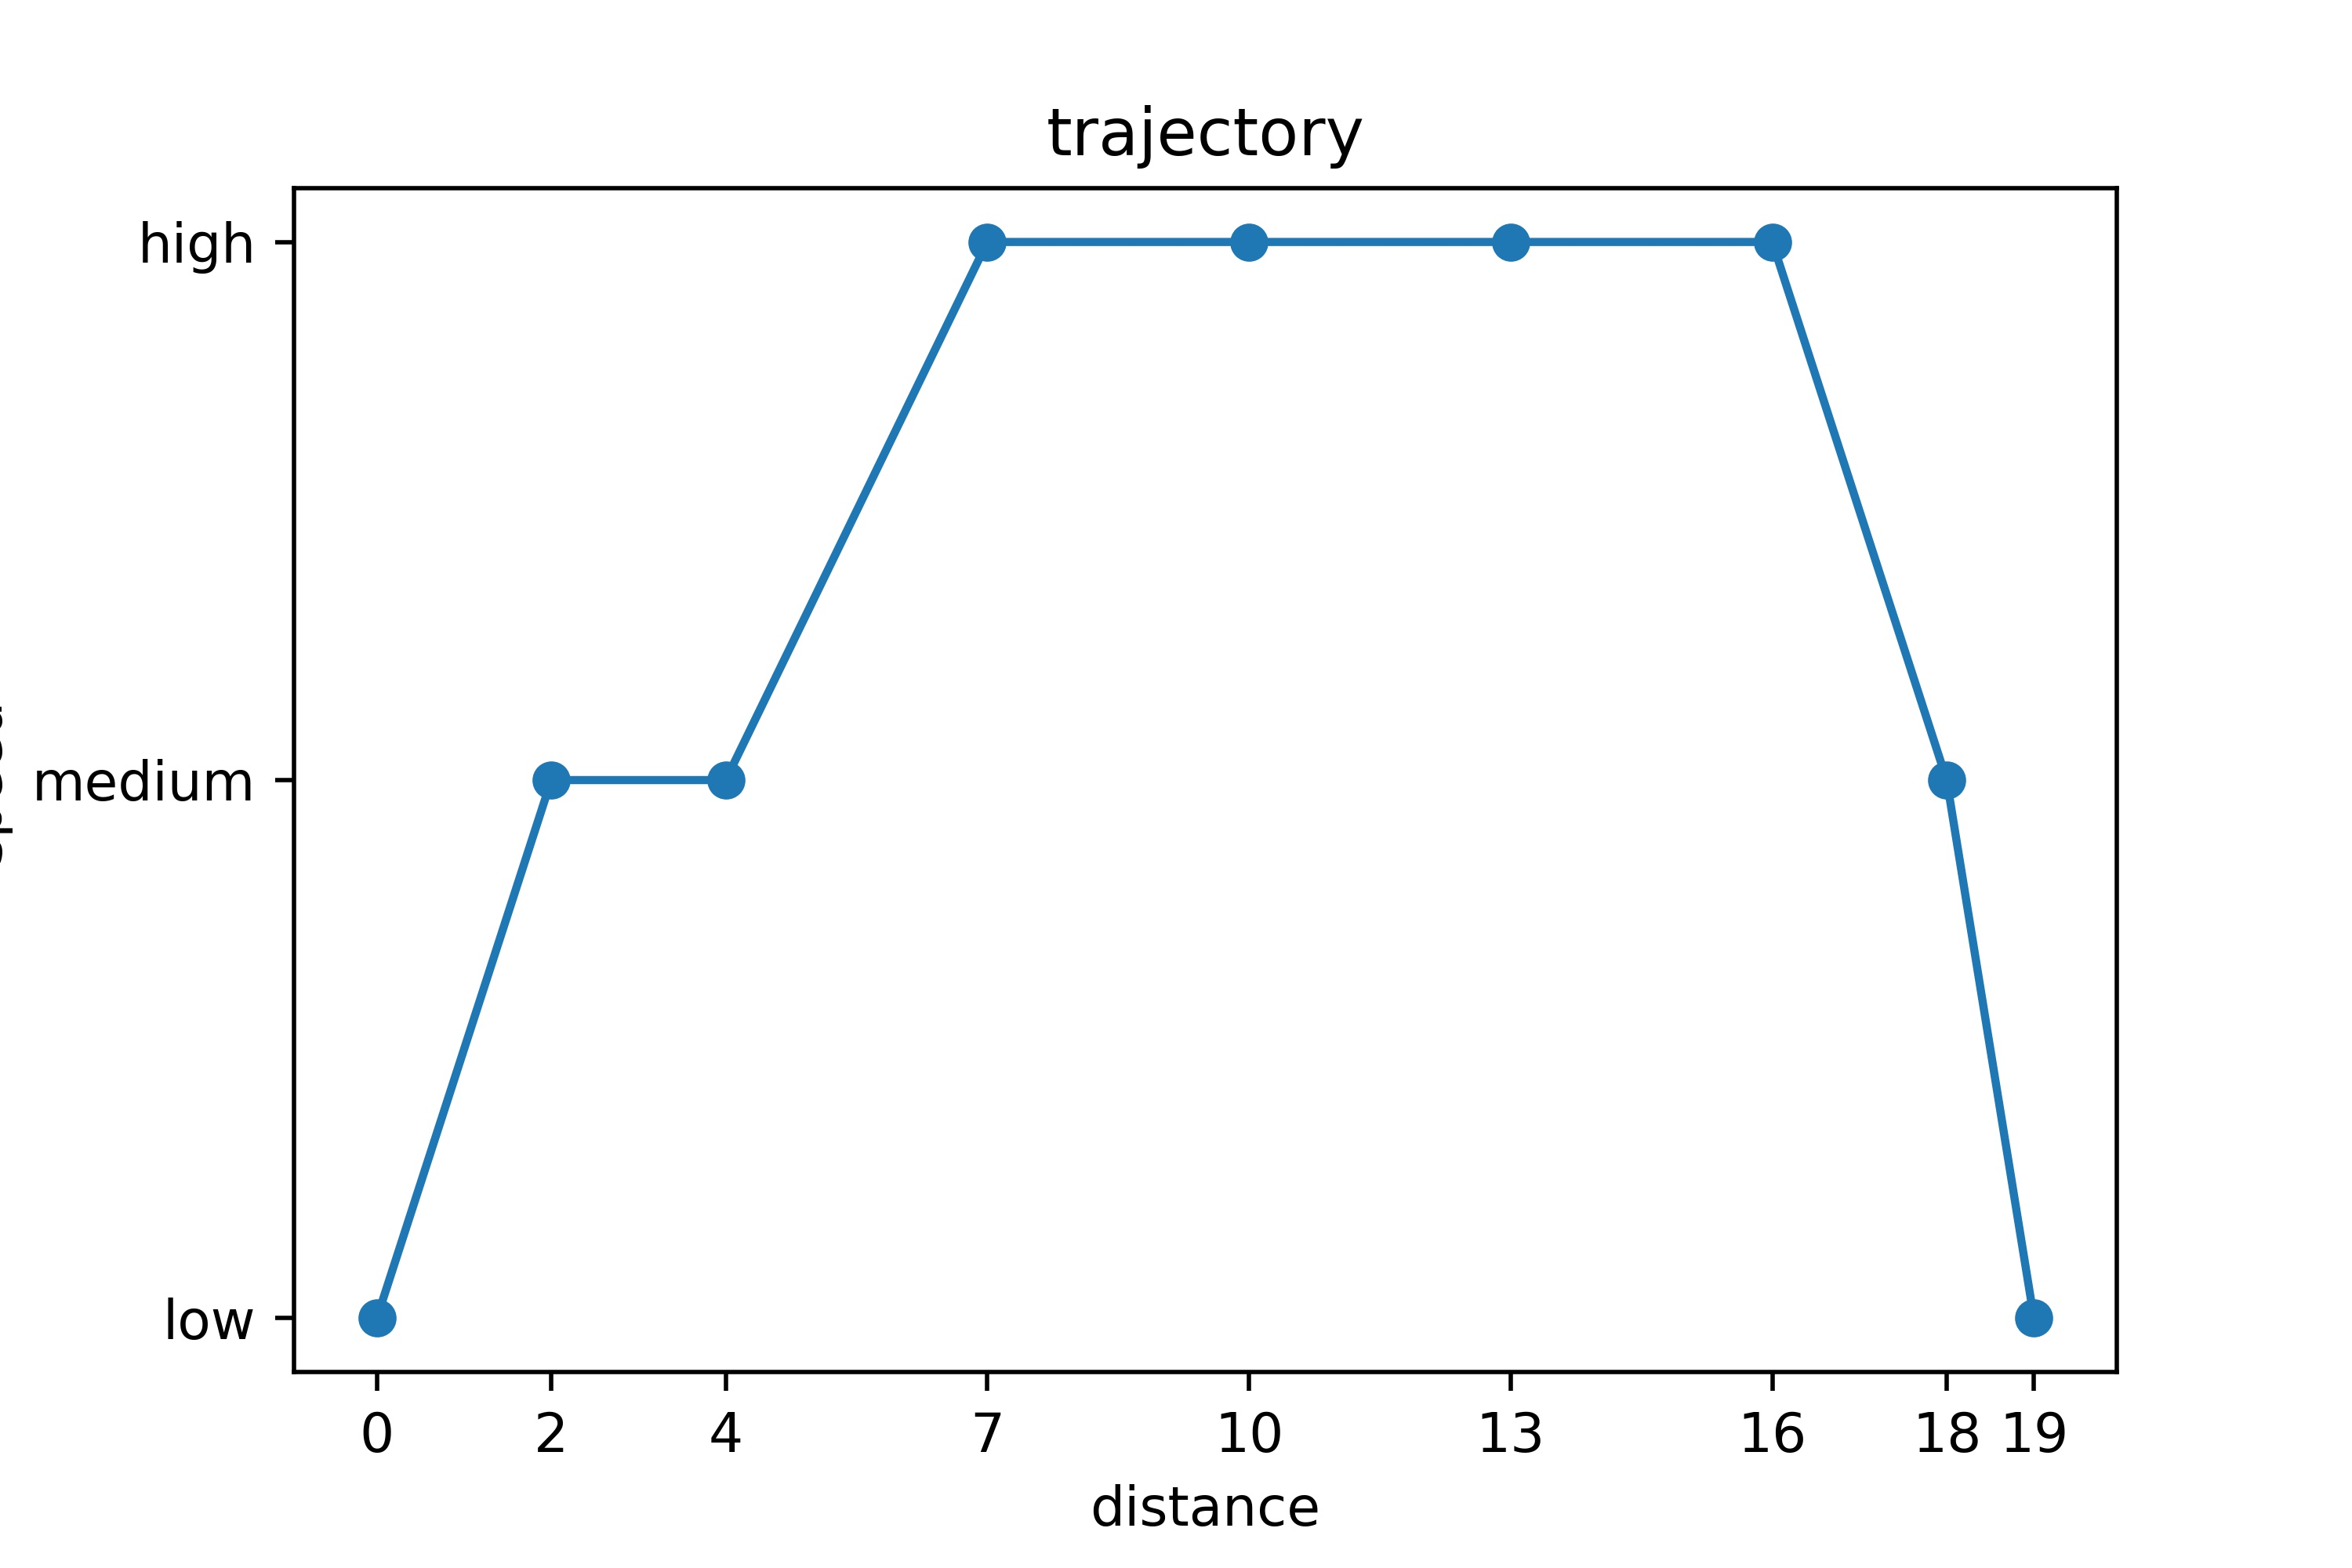
\includegraphics[scale=0.5]{img/trajectory.jpg}
\end{frame}

\begin{frame}
\frametitle{Results when uncertainty introduced into brakes}
\framesubtitle{Evolution of the trajectories during iteration 0,2, and 4 (optimal)}
\centering
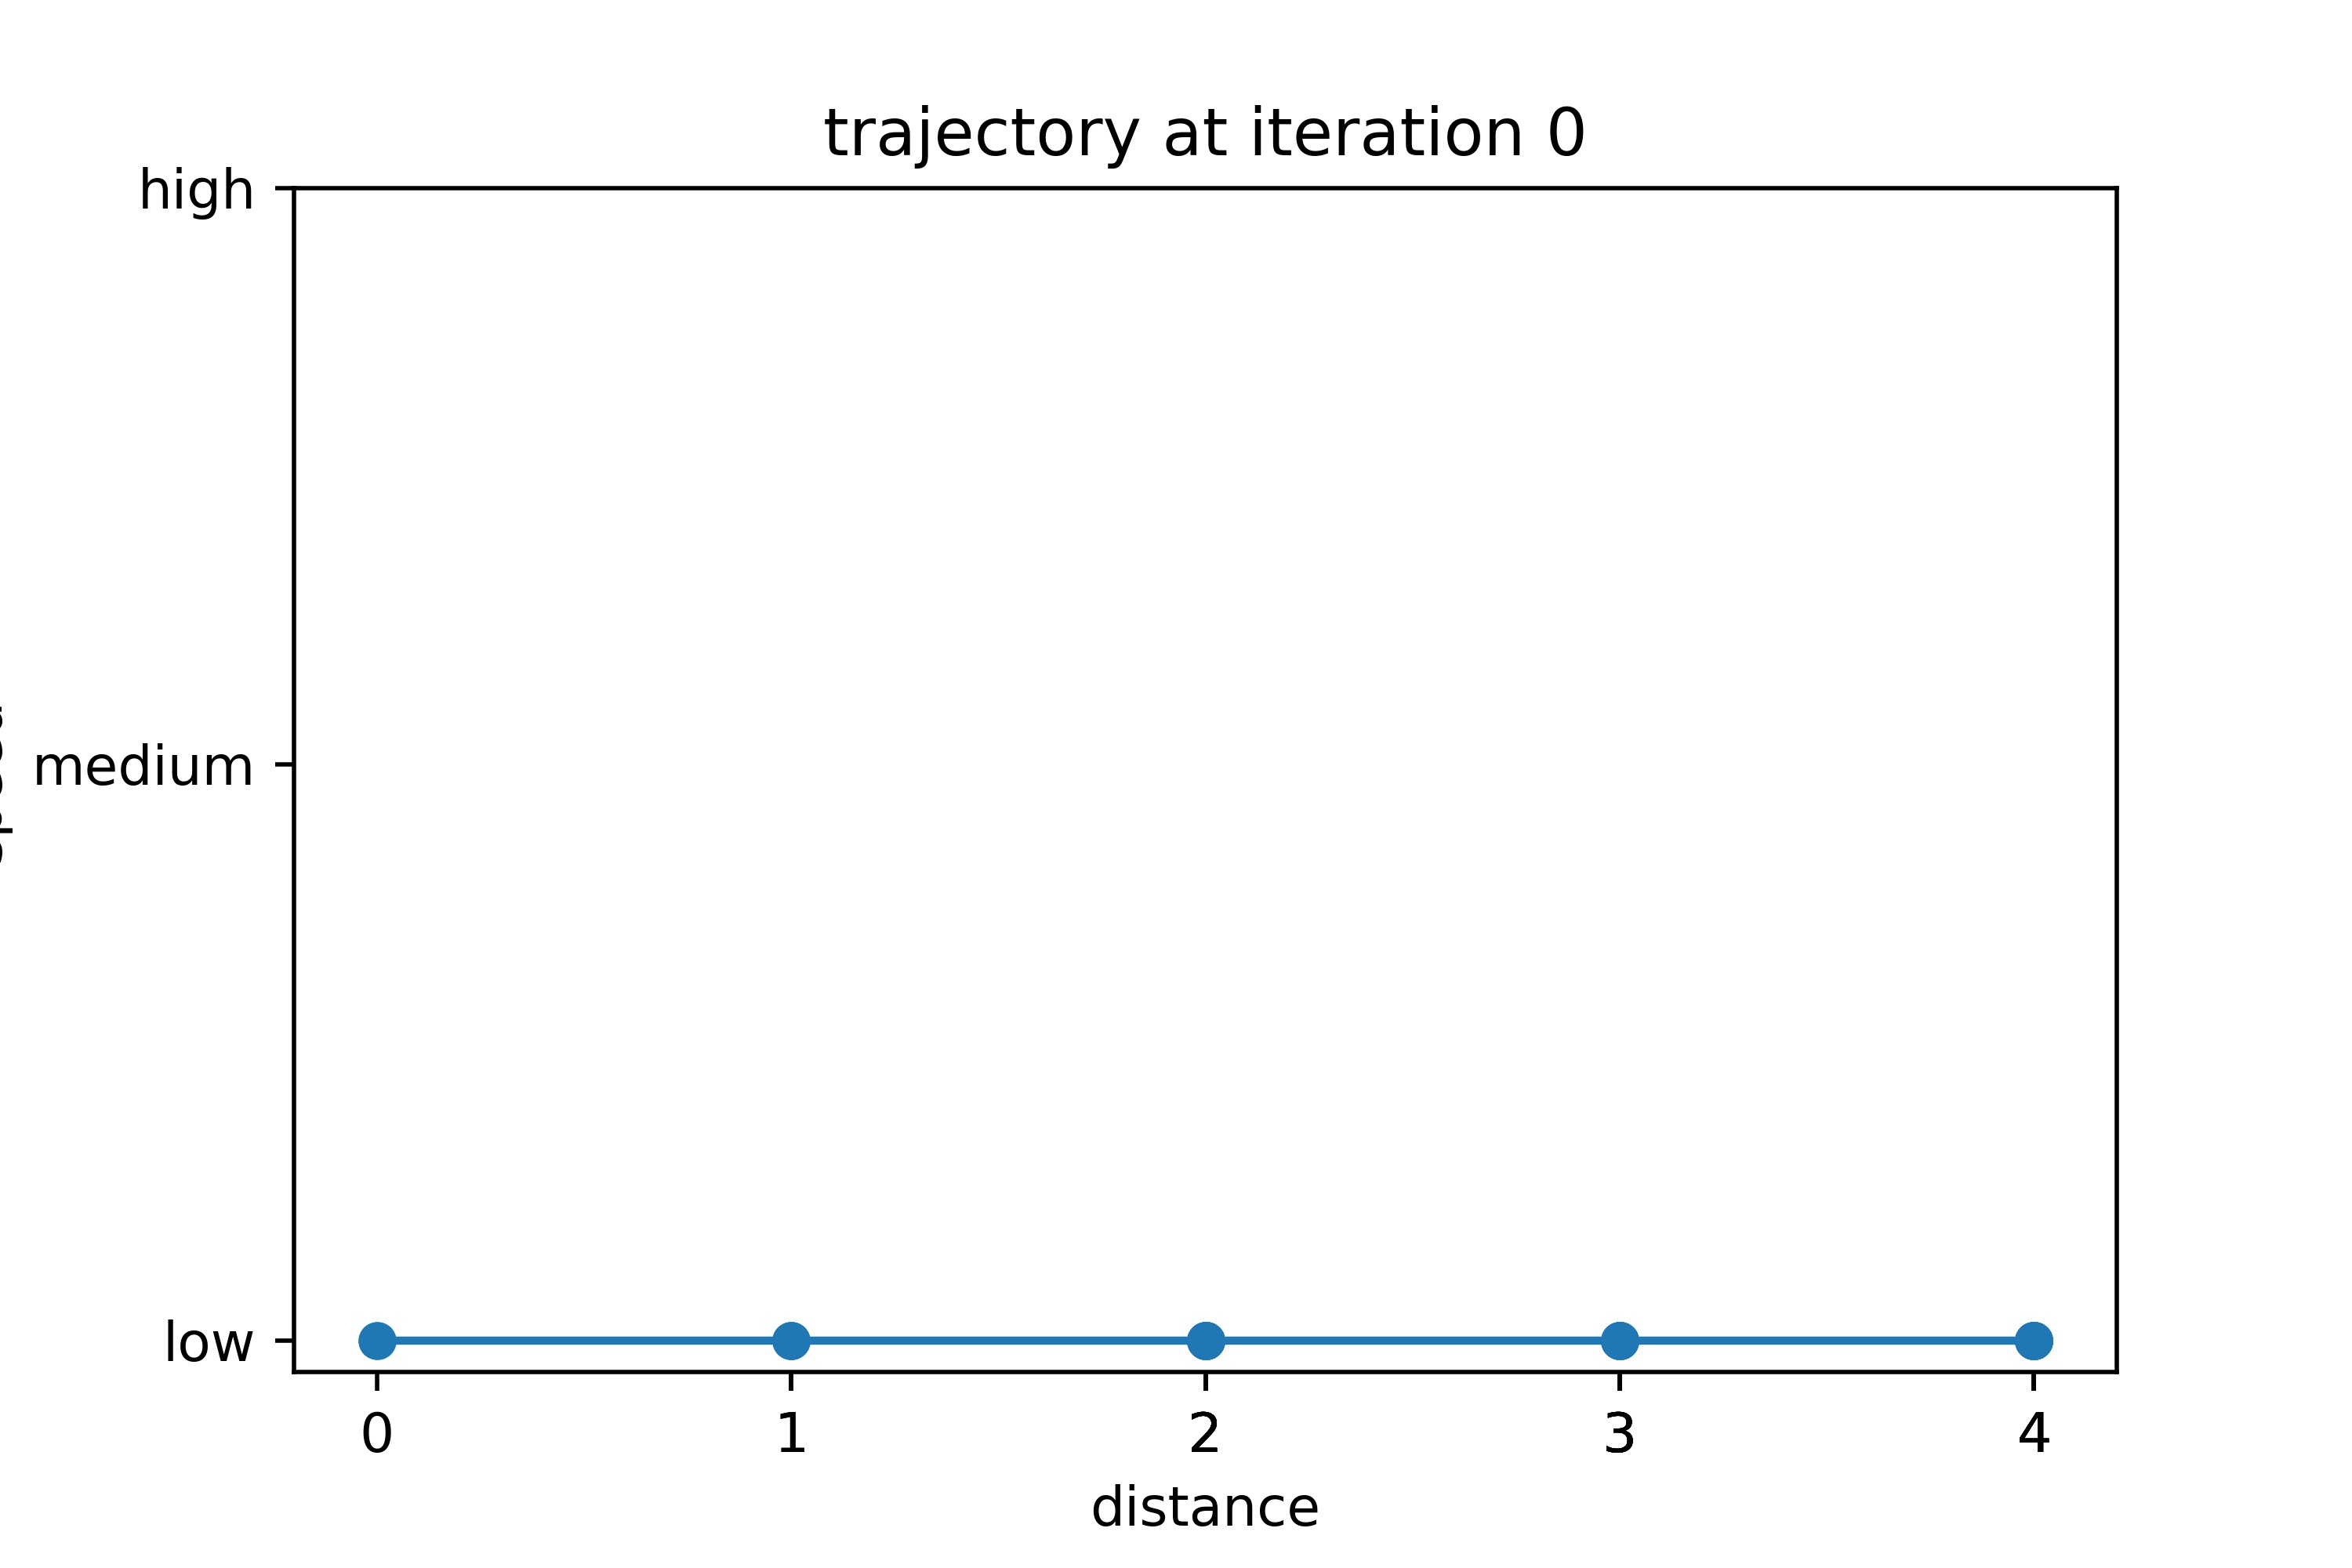
\includegraphics[scale=0.35]{img/trajectory0.jpg}
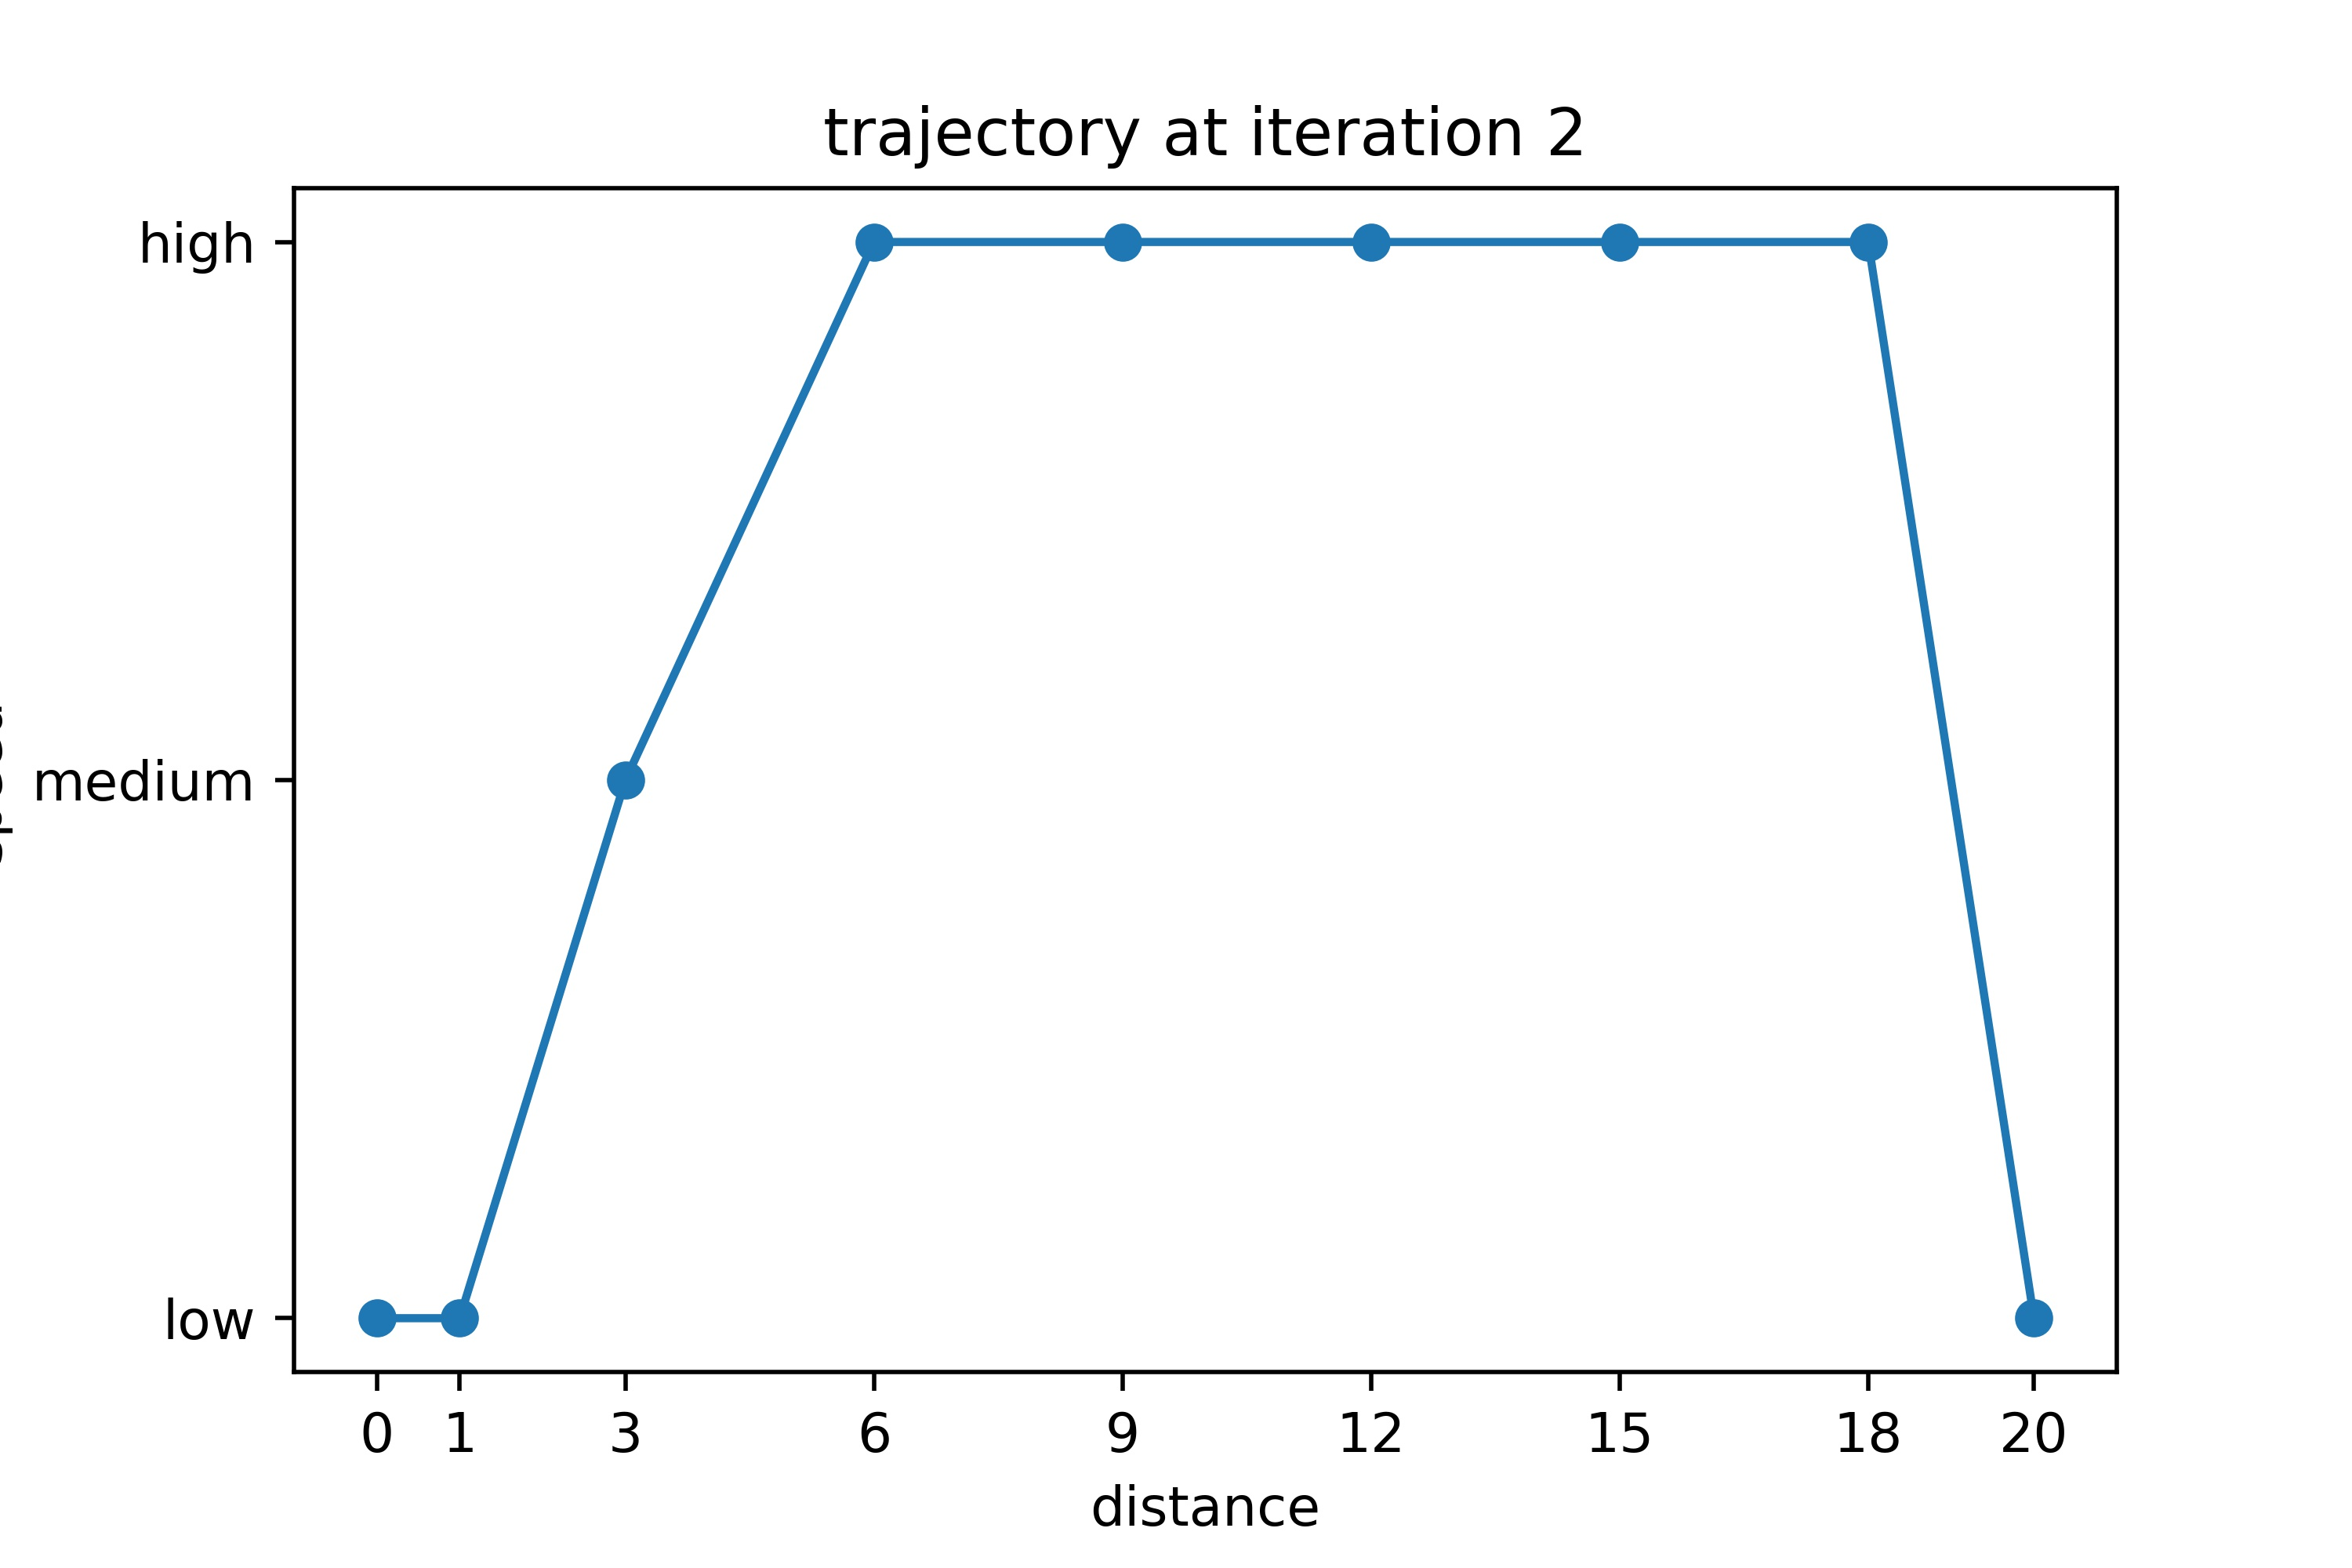
\includegraphics[scale=0.35]{img/trajectory2.jpg}
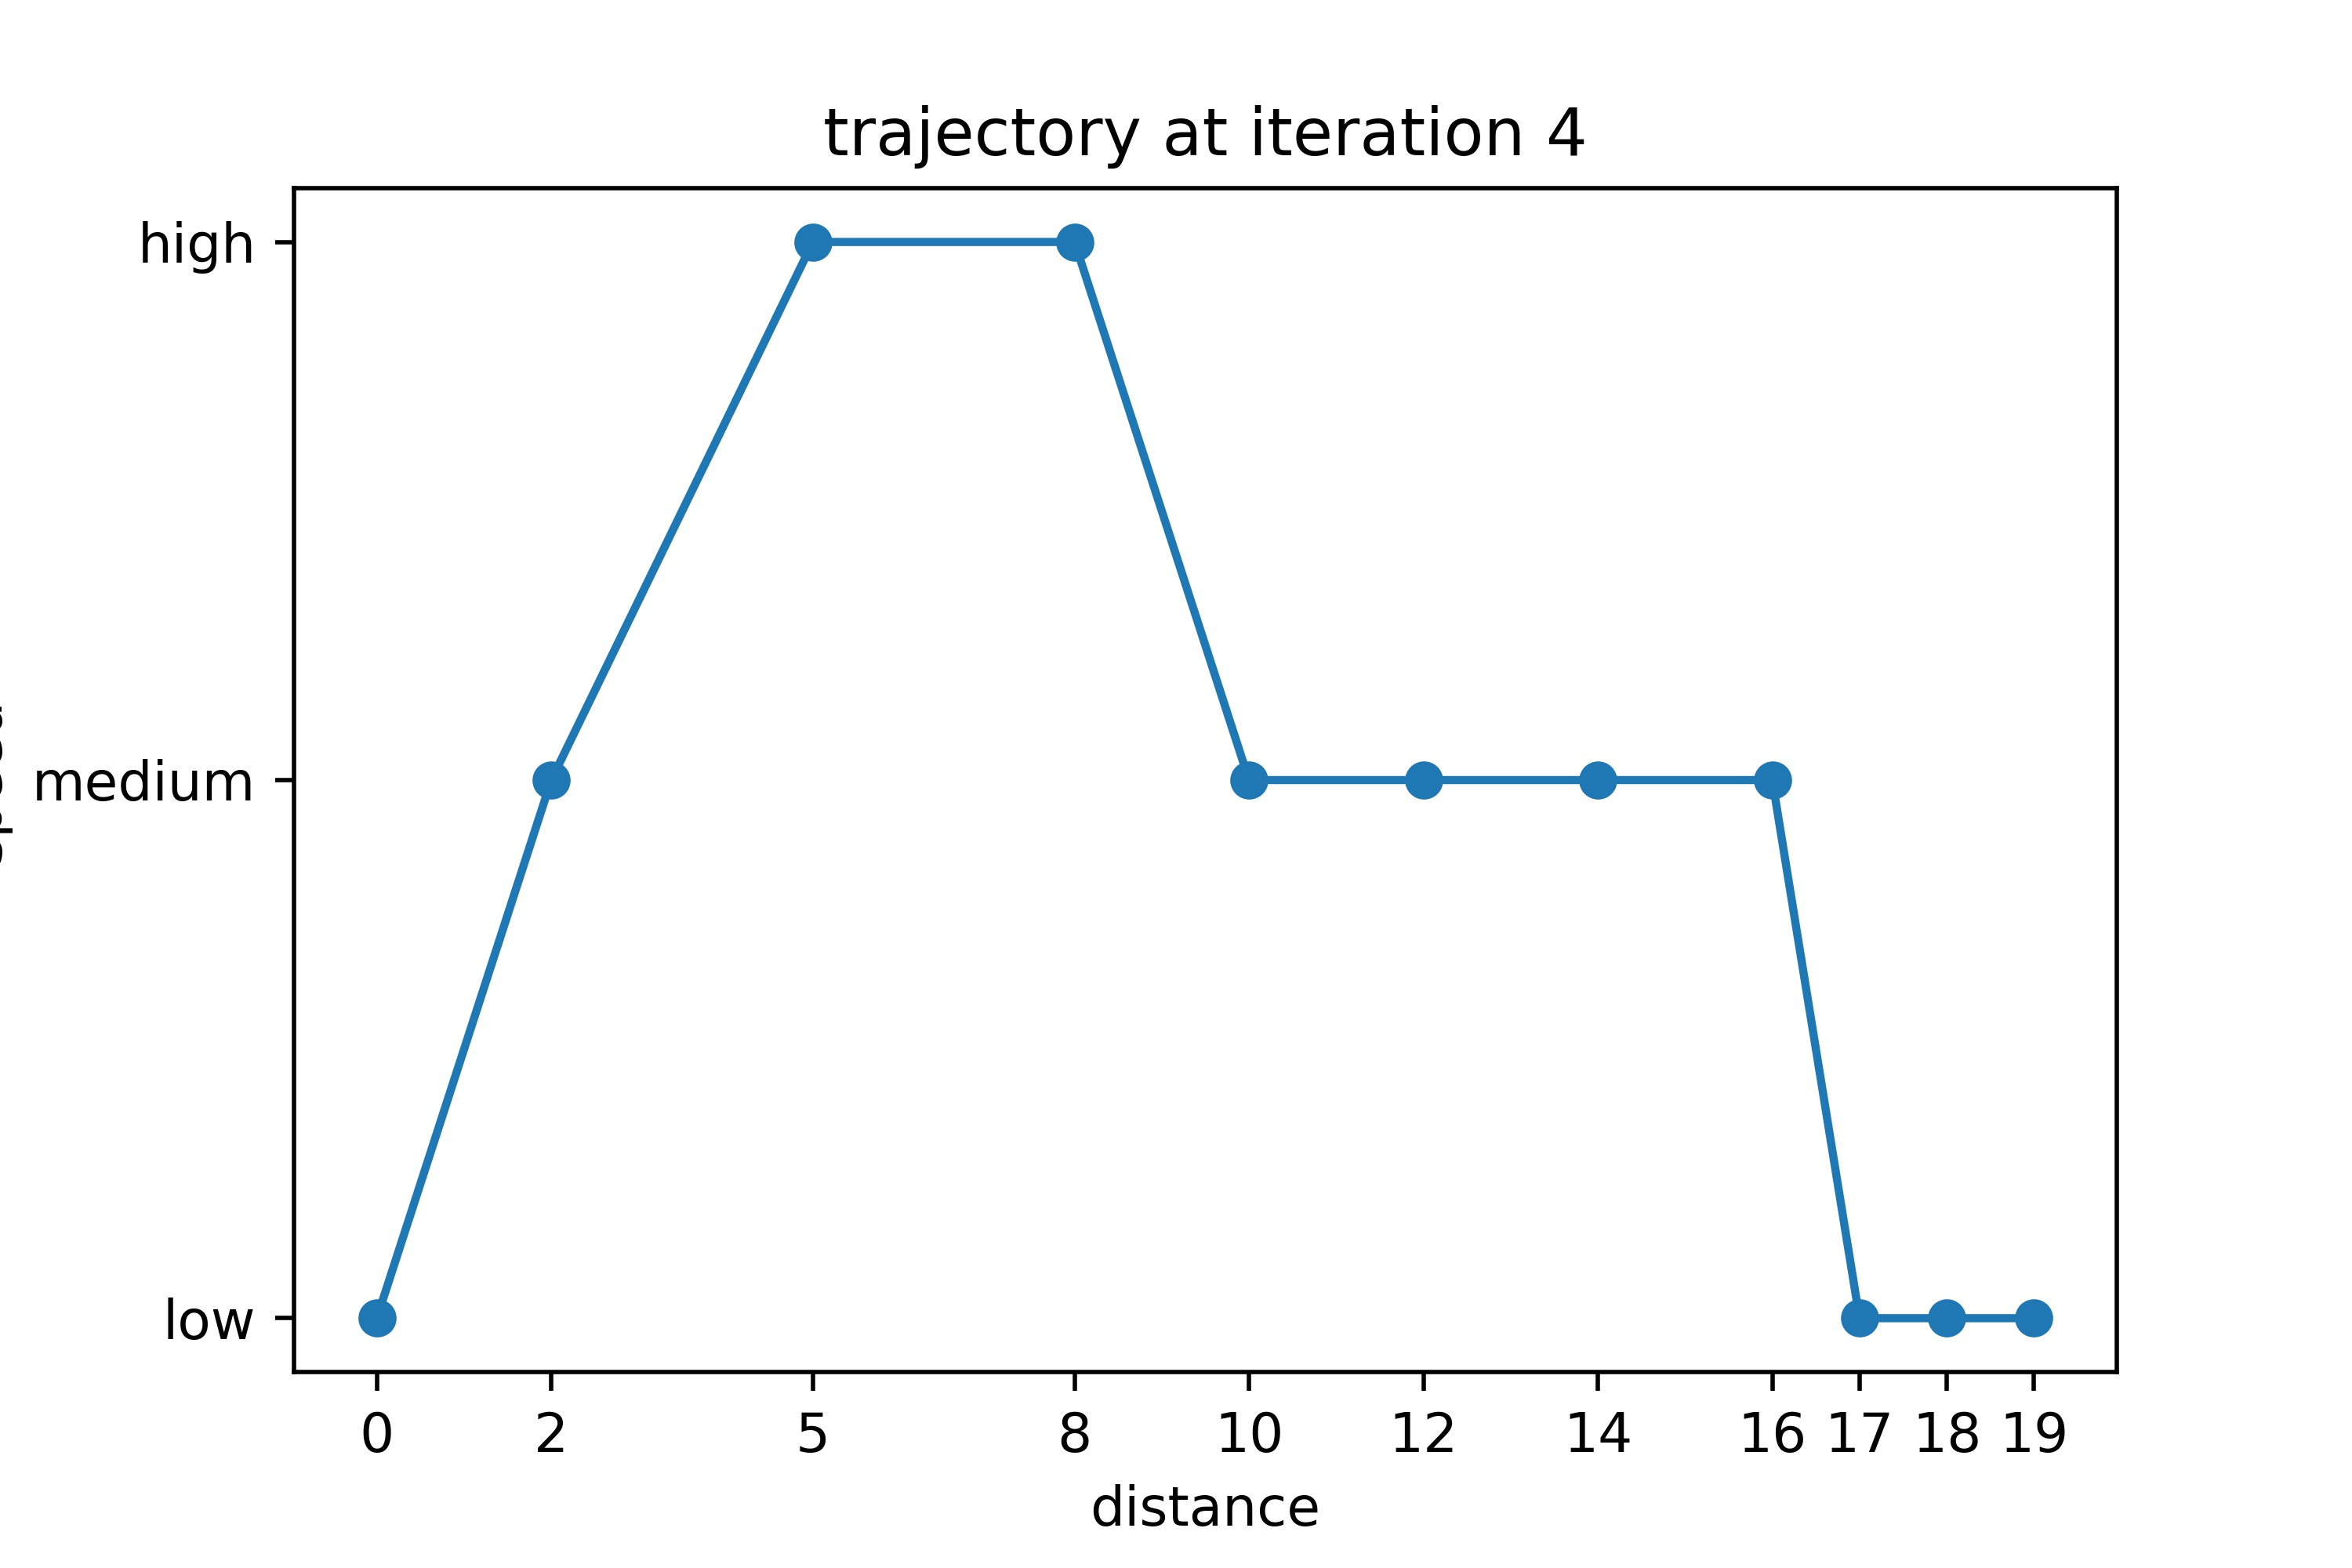
\includegraphics[scale=0.35]{img/trajectory4.jpg}
\end{frame}

\begin{frame}
\frametitle{Conclusion, what have we done ? }
\begin{block}{}
\begin{itemize}
\item We introduced the theoretical framework,the Markov Decision Process
\item We solved a simple problem where we know the model
\end{itemize}
\end{block}
\end{frame}



\begin{frame}
\frametitle{What's next ? }



\begin{block}{already working on}
\begin{itemize}
\item Add the traffic light into this setting
\item Find the distance from the robot's camera to the traffic light
\end{itemize}
\end{block}

\begin{block}{In a not so distant future}
\begin{itemize}
\item explore other algorithm and compare them : Monte-Carlo methods, temporal difference learning, Q learning, $\ldots$
\item Neuro-dynamic programming ?
\end{itemize}
\end{block}

\pause
\begin{block}{Ultimately}
Implement everything on the robot ... \pause and pray that everything works well
\end{block}

\end{frame}




\end{document}
